%!TEX TS-program = xelatex
\documentclass[]{friggeri-cv}
\usepackage{afterpage}
\usepackage{hyperref}
\usepackage{color}
\usepackage{xcolor}
\hypersetup{
    pdftitle={},
    pdfauthor={},
    pdfsubject={},
    pdfkeywords={},
    colorlinks=false,       % no lik border color
   allbordercolors=white    % white border color for all
}
\addbibresource{bibliography.bib}
\RequirePackage{xcolor}
\definecolor{pblue}{HTML}{0395DE}

\begin{document}
\header{Tyler }{ Lyle}
      {Software Developer}
      
% Fake text to add separator      
\fcolorbox{white}{gray}{\parbox{\dimexpr\textwidth-2\fboxsep-2\fboxrule}{%
.....
}}

% In the aside, each new line forces a line break
\begin{aside}
  \section{Address}
    2115 New Road
    Waterford, PA 16441
    ~
  \section{Telephone}
    +1 (814) 464 3068
    ~
  \section{Mail}
    \href{mailto:}{\textbf{jobsearch\_lylet@}\\yahoo.com}
    ~
  \section{Web \& Git}
    \href{https://tyler-lyle.netlify.com/}{tyler-lyle.netlify.com}
    \href{https://bitbucket.org/tylerlyle}{bitbucket.org/\textbf{tylerlyle}}
    \href{https://github.com/lylet-AC}{github.com/\textbf{lylet-AC}}
    ~
  \section{Programming}
    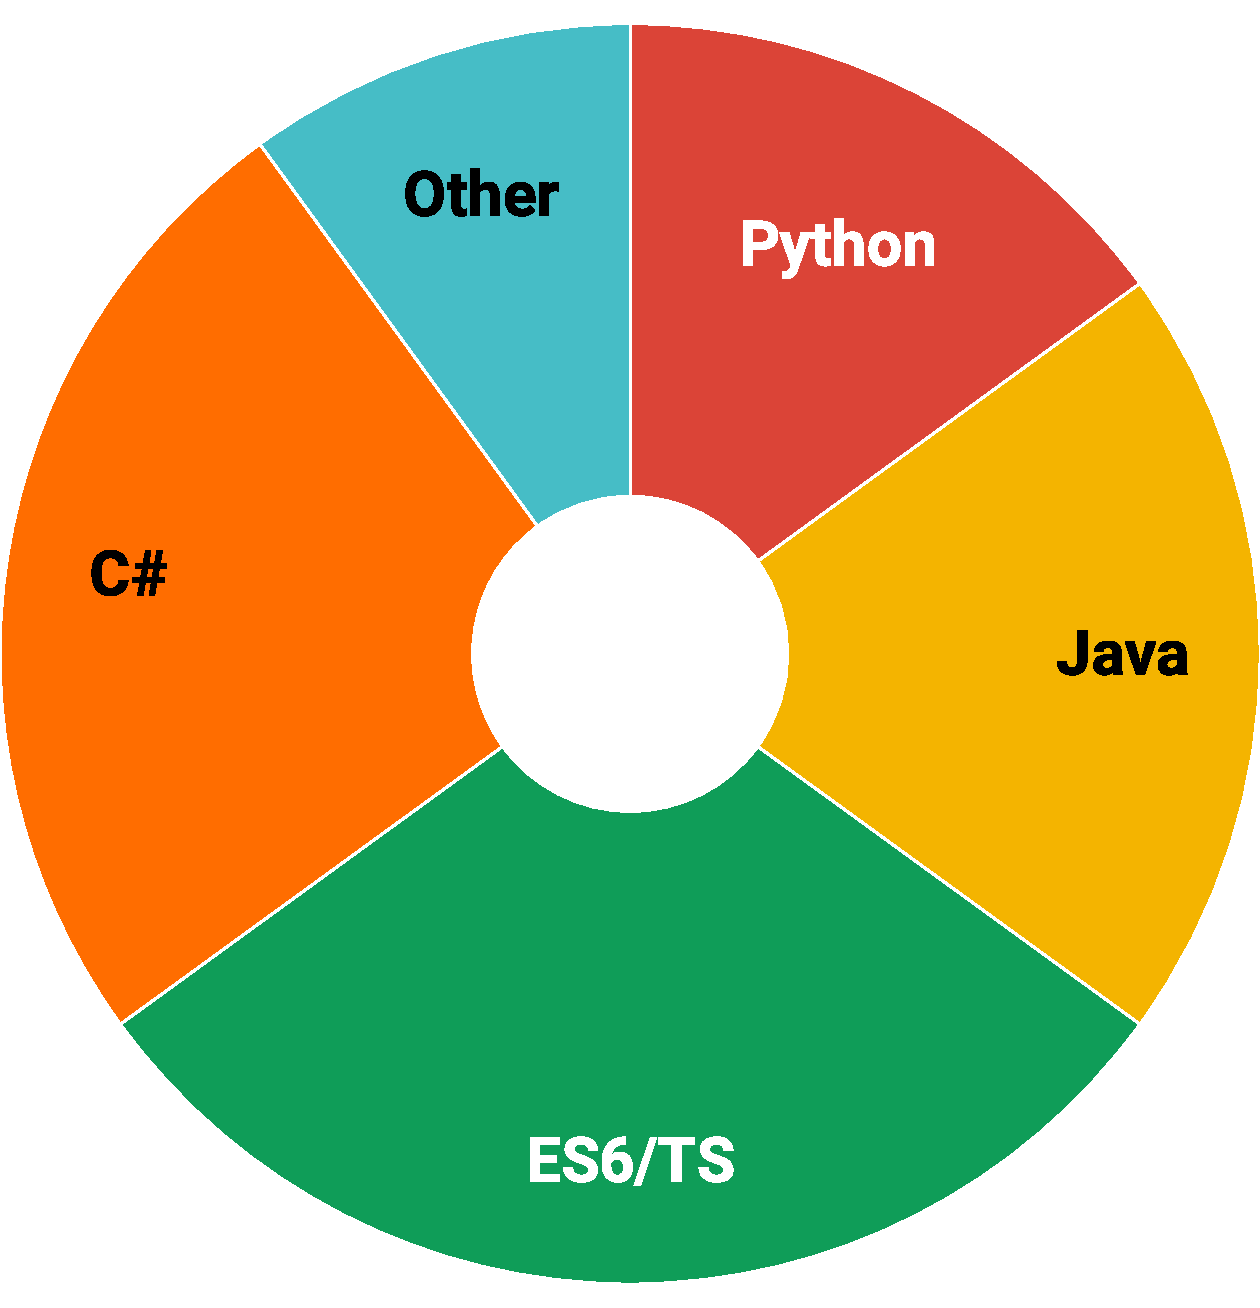
\includegraphics[scale=0.18]{img/pvl.pdf}
    ~
  \section{OS Preference}
    \textbf{GNU/Linux}
\includegraphics[scale=0.40]{img/5stars.png}
    \textbf{MacOS}
\includegraphics[scale=0.40]{img/3stars.png}
    \textbf{Windows}
\includegraphics[scale=0.40]{img/4stars.png}
    ~
  \section{Personal Skills}
    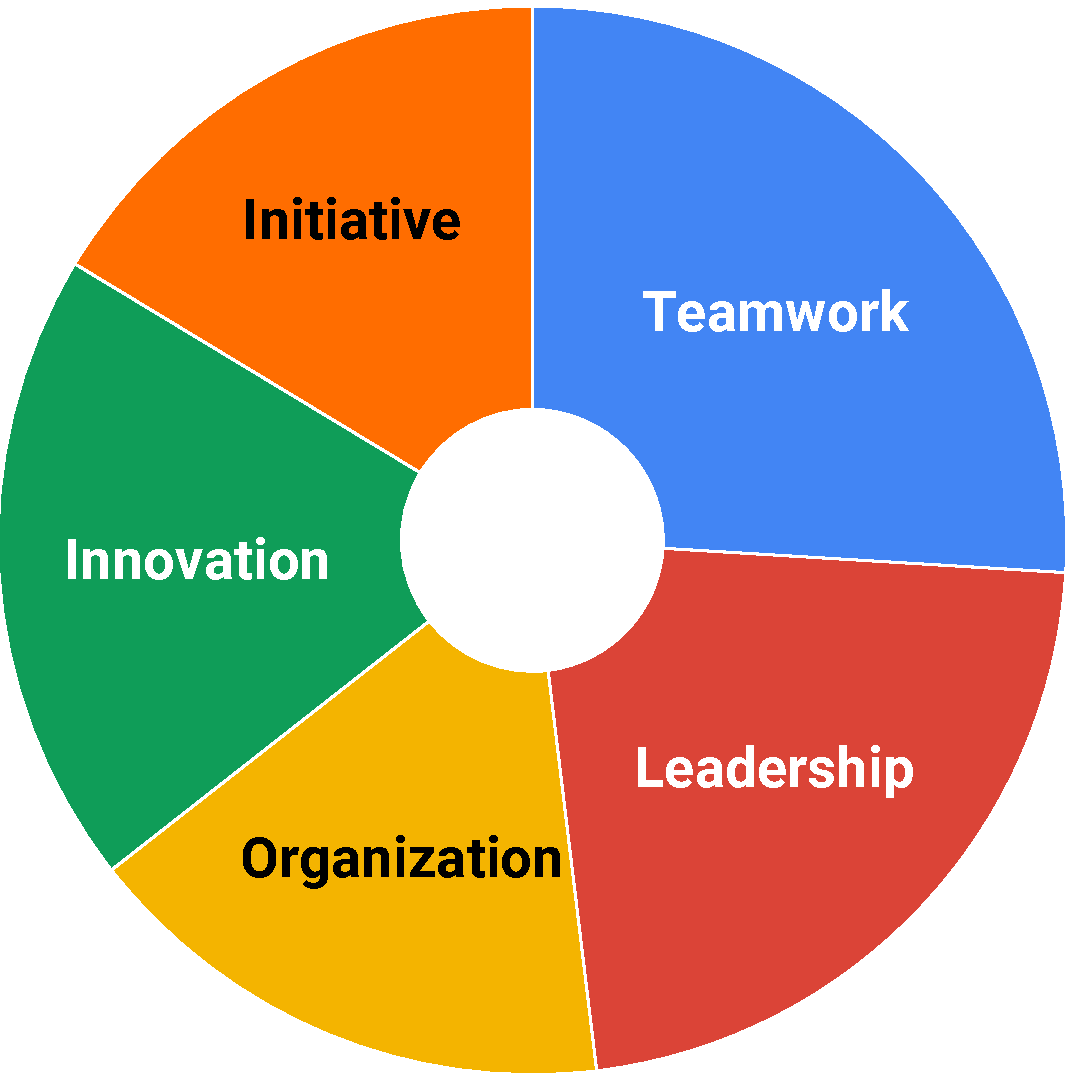
\includegraphics[scale=0.2]{img/skills.pdf}
    ~
\end{aside}

\section{About Me}
\begin{entrylist}
	\entry
	{}
	{Computer Enthusiast}
	{First Generation College Student}
	{
		I always have had a fascination with computer programming.  Starting from age 10 armed with an Ubuntu powered laptop, I began my journey as software developer. This passion has met a recent apex when I graduated from Allegheny College in May of 2019.  However, this is not the end of my journey as I wish to continue my passion in the industry of software engineering.

	}
\end{entrylist}

\section{Education}
\begin{entrylist}
	\entry
	{2015 - 2019}
	{Bachelor's Degree in Computer Science}
	{Allegheny College}
	{Software Engineering.\\
		Main subjects: Software Engineering, Artificial Intelligence, Distributed Cloud Systems, Web Development.\\
	}
	
	\entry
	{2011 - 2015}
	{High School Diploma}
	{McDowell High School}
	{Secondary School.\\
		Main subjects: Computer Science, Game Design, AutoCAD, Engineering.\\}
\end{entrylist}

\section{Software Projects}
\begin{entrylist}
	\entry
	{}
	{GatorGrader}
	{Allegheny College}
	{Python tool for the automated grading of Computer Science projects hosted on GitHub. \emph{Relator: Dr. Gregory Kapfhammer.}\\}
	
	\entry
	{}
	{Pynesthesia}
	{Allegheny College}
	{Python project which allows for the creation of a simple tile based game using an image as the input. \emph{Relators: Prof. Janyl Jumadinova, Prof. Aravind Mohan.}\\}
	
	\entry
	{}
	{Ardbot}
	{Allegheny College}
	{A multi-state robotic client designed for the autonomous playing of the popular e-sport game Rocket League. \emph{Relators: Prof. Janyl Jumadinova.}\\}
	
\end{entrylist}

\section{Work Experience}
\begin{entrylist}
  \entry
    {6/17 - Now}
    {POS Operator}
    {Kohl's Department Store}
    {Guarantee customer satisfaction, solicit Kohl's Charge store cards, cash out customers, evening cash management.\\}
  \entry
    {6/13 - 2/18}
    {Shift Supervisor \& Closing Manager}
    {The Wendy's Company}
    {Ensure that food meets safety and quality standards, conduct interviews, train crew members, evening cash management, nightly inventory audits, establish goals.\\}
\end{entrylist}

\begin{flushleft}
\emph{April 21st, 2019}
\end{flushleft}
\begin{flushright}
\emph{Tyler Lyle}
\end{flushright}

\end{document}
